\documentclass{spisok-article}

\usepackage{amsmath,amsthm}
\usepackage{amsfonts,amssymb}
\usepackage{listings}

\newtheorem{definition}{Определение}

\title{О распараллеливании метода численного нахождения ляпуновских экспонент с помощью OpenMP}

\author{Бурова И. Г., д.ф.-м.н, проф. СПбГУ 

Мокаев Т. Н., к.ф.-м.н., мл. науч. сотр. СПбГУ

Федоров Е. Г., студент мат.-мех. факультета СПбГУ}

\begin{document}

\maketitle

\begin{abstract}
В данной статье описан метод нахождения ляпуновских показателей с помощью алгоритма Бенеттина. А также сравнивается время вычисления при последовательной и параллельной реализациях множественного запуска данного алгоритма.
\end{abstract}

\section{Введение}
Ляпуновские показатели являются важными числовыми характеристиками динамической системы. Нередко необходимо вычислять эти показатели для большого количества траекторий, например при оценке ляпуновской размерности инвариантного множества~\cite{book:strange_attractors, art:kuznetsov_lyapunov_dim}. Из-за большой вычислительной сложности алгоритма, это может занять много времени. Для ускорения вычислений можно воспользоваться стандартом $OpenMP$ для распараллеливания программы, распределив траектории по разным потокам.

\section{Определение ляпуновских показателей}

Дадим определение ляпуновских показателей в соответствии с работами~\cite{art:lyapunov_exp, art:CNSNS_2014}.

Пусть дана система дифференциальных уравнений

\begin{equation} \label{eq:diff}
\frac{dx}{dt} = f(x), t \in \mathbb{R}, x \in U,
\end{equation}
где $U$ --- открытое подмножество $\mathbb{R} ^n$ ($U \subseteq \mathbb{R} ^n$), $f$ непрерывно дифференцируемая вектор функция $U \to \mathbb{R} ^n$. Пусть $\varphi (t, x_0)$ --- решение этой системы такое, что $\varphi (0,x_0) = x_0$.

Рассмотрим линеаризацию системы~(\ref{eq:diff}) вдоль решения $\varphi (t,x_0)$:
\begin{equation} \label{eq:linear}
\dot{y} = J(\varphi (t,x_0)) y, \quad J(x) = D f(x),
\end{equation}
где $J$ --- $n \times n$ матрица Якоби. Пусть $D(\varphi (t,x_0)) = \left (y_1 (t,x_0), \ldots y_n(t,x_0) \right )$ фундаментальная матрица линеаризованной системы~(\ref{eq:linear}) такая, что $D(\varphi (0,x_0)) = I$, где $I$ --- единичная $n \times n$ матрица. Теперь можно ввести следующее определение:

\begin{definition} \label{def:lce}
Ляпуновским показателем $\mu _i (x_0)$ называется число $$\mu _i (x_0) = \varlimsup \limits _{t \rightarrow +\infty} \frac{1}{t} ln \left \| y_i (t,x_0) \right \|.$$

Показатель $\mu _i (x_0)$ называется строгим, если существует конечный предел $$\mu _i (x_0) = \lim \limits _{t \rightarrow +\infty} \frac{1}{t} ln \left \| y_i (t,x_0) \right \|.$$
\end{definition}

\section{Алгоритм Бенеттина}

Дадим краткое описание алгоритма Бенеттина~\cite{art:alg_benettin_teory, art:alg_benettin_app} для численного нахождения ляпуновских показателей траектории системы~(\ref{eq:diff}). Запишем вариационное уравнение системы~(\ref{eq:diff}) в следующем виде

\begin{equation} \label{eq:var}
\dot{X} = JX,
\end{equation}
где $X$ --- $n \times n$ матрица, $J$ --- якобиан функции $f$.

Пусть $x_0$ --- начальная точка траектории, $Q_0 = I$, где $I$ --- единичная $n \times n$ матрица. На $i$-ой итерации алгоритма исходная система~(\ref{eq:diff}) и её вариационное уравнение~(\ref{eq:var}) интегрируются с начальными данными $(x_{i-1}, Q_{i-1})$ на временном интервале $\left ( ih-h, ih \right )$, где $h$ --- малый интервал времени, параметр алгоритма. Обозначим результат интегрирования, как $(x_i, H_i)$. Затем матрица $H_i$ $QR$-факторизуется: $H_i = Q_i R_i$. Для следующей итерации используется пара $(x_i, Q_i)$. Количество итераций $N$, также является параметром алгоритма.

В результате численную оценку $j$-ого ляпуновского показателя можно записать как
\begin{equation} \label{eq:number_lce}
\mu _{j} (x_0) = \frac{1}{Nh} \sum \limits _{i=1} ^{N} \ln(R_i (j,j))
\end{equation}

Определение ляпуновских показателей и алгоритм их численного нахождения приведены только для направлений ортов декартовой системы, но также возможно обобщение для $n$ линейно независимых векторов.

\section{Сравнение последовательной и параллельной реализации}
Для вычисления ляпуновских показателей были написаны последовательная и параллельная
  реализации на языке $C++$. Для распараллеленной реализации использовался открытый стандарт $OpenMP$ (Open Multi-Processing). А именно, директивы $parallel$ для создания потоков, директивы $for$ для распределения вычислений по потокам, а также конструкции $shared$ и $private$ для задания типа переменных, используемых в параллельных секциях.



Пример части параллельной реализации:

\begin{lstlisting}[language=C]
#pragma omp parallel for shared(result_lces) num_threads(NUM_THREADS)
for (int iteration = 0; iteration < COUNT_POINTS; ++iteration)
{
    result_lces[iteration] = computeLCEs(system, dimension,
        POINTS[iteration], COUNT_ITERATIONS, D_TIME);
}
\end{lstlisting}

Обе реализации запускались с помощью компилятора из среды \emph{Visual Studio 2013}. Операционная система \emph{Windows 8.1}. Характеристики компьютера: 4-x ядерный
процессор \emph{Intel Core i5-5200U 2.20 GHz}.

Будем называть коэффициентом ускорения отношение времени работы распараллеленной
реализации к последовательной. Теоретически коэффициент ускорения не может быть больше, чем
$\frac{1}{\alpha+\frac{1-\alpha}{N}}$, где $\alpha$ доля расчетов, которые могут
быть получены только последовательными вычислениями. На практике этот коэффициент
еще меньше за счет накладных расходов на создание и содержание нескольких потоков
вычисления, за счет окончательного формирования результатов по завершению
вычислений во всех потоках. А также на коэффициент ускорения влияет загруженность
процессора в данный момент задачами не относящимися к данной.

Для численного эксперимента была рассмотрена обобщенная система Лоренца~\cite{art:rabinovich_main, art:lyap_meth_for_hausd_dim, art:CNSNS_2014, art:EPJST_2015}:

\begin{equation} \label{eq:lorenz}
\left\{
\begin{array}{rcl}
  \dot x & = & -\sigma (x-y)-ayz \\
  \dot y & = & rx-y-xz \\
  \dot z & = & -bz+xy
\end{array}
\right.,
\end{equation}
со значениями параметров $\sigma = 4, a = -0.66, r = 6.05, b = 1$.

Далее приведены четыре графика зависимости коэффициента ускорения 
от $n$ --- количества траекторий. Два графика соответствуют запуску на два потока, два других --- на четыре потока. Параметры алгоритма: $1000$ --- количество итераций, $0.1$ --- временной шаг.

\begin{figure}[h]
    \begin{center}
        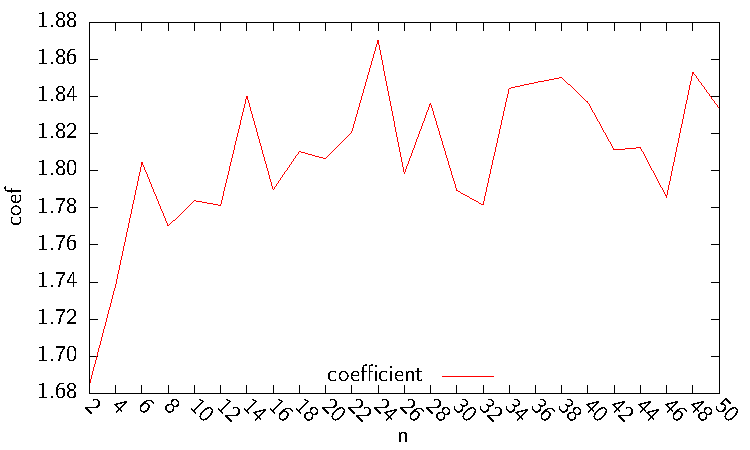
\includegraphics[width=0.9\textwidth]{plot_2-1.pdf}
    \end{center}
    \caption{Два потока, первый запуск}\label{fig:two_threads_1}
\end{figure}

\begin{figure}[hp!]
    \begin{center}
        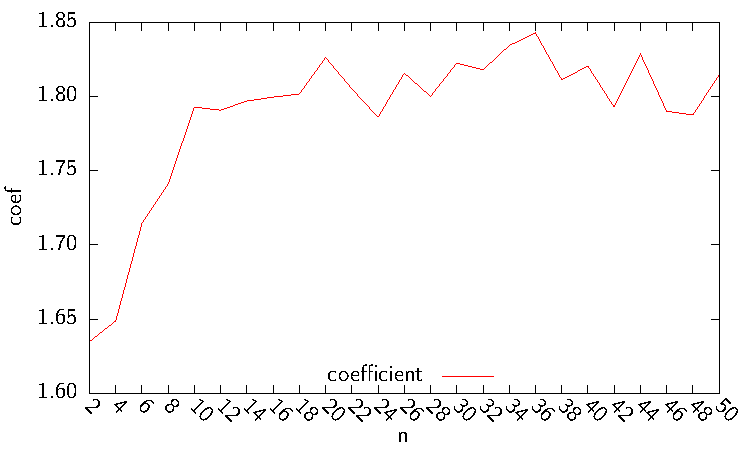
\includegraphics[width=0.9\textwidth]{plot_2-2.pdf}
    \end{center}
    \caption{Два потока, второй запуск}\label{fig:two_threads_2}
\end{figure}

\begin{figure}[hp]
    \begin{center}
        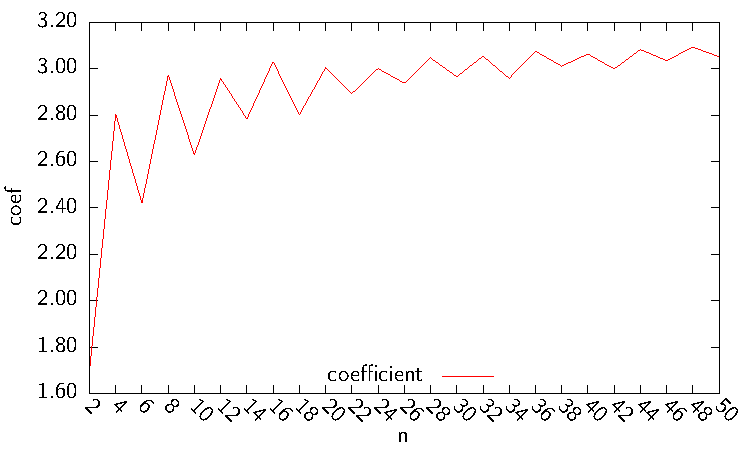
\includegraphics[width=0.9\textwidth]{plot_4-1.pdf}
    \end{center}
    \caption{Четыре потока, первый запуск}\label{fig:four_threads_1}
\end{figure}

\begin{figure}[hp]
    \begin{center}
        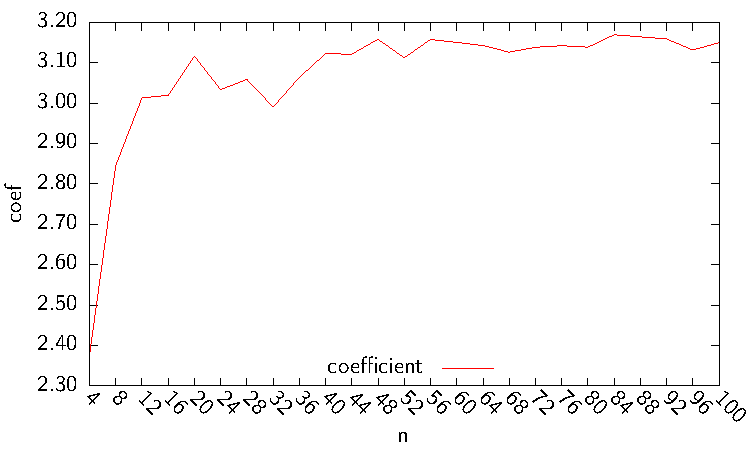
\includegraphics[width=0.9\textwidth]{plot_4-2.pdf}
    \end{center}
    \caption{Четыре потока, второй запуск}\label{fig:four_threads_2}
\end{figure}

Для уменьшения влияния внешних факторов на коэффициент ускорения для каждого $n$ последовательная и параллельная реализации запускались по очереди 100 раз. Коэффициент ускорения вычислялся как отношение суммарного времени работы всех запусков последовательной реализаций к аналогичному показателю параллельной реализации.

Как видно из графиков, с ростом $n$ растет и коэффициент ускорения, т.е. накладные расходы на создание и содержание потоков становятся менее значительными. Также видно, что при достаточно большом $n$ параллельная реализация на четырех потоках работает в три раза быстрее, чем последовательная, что является значительным ускорением времени работы.

\section{Заключение}
В данной работе было дано определение ляпуновских показателей и описан алгоритм Бенеттина для их численного нахождения. Также показано, что с помощью $OpenMP$ можно добиться значительного уменьшения времени работы программы.

\renewcommand\refname{Литература}
\begin{thebibliography}{8}

\bibitem{book:strange_attractors} {\it Леонов Г.\;А.} Странные аттракторы и классическая теория устойчивости движения. — Изд-во СПбГУ СПб., 2004.

\bibitem{art:kuznetsov_lyapunov_dim} {\it Kuznetsov N.\;V.} The Lyapunov dimension and its estimation via the Leonov method // Physics Letters A. --- 2016.

\bibitem{art:lyapunov_exp} {\it Lyapunov A.\;M.} The general problem of the stability of motion // International Journal of Control. --- 1992. --- Vol. 55, no. 3. --- P. 531--534.

\bibitem{art:CNSNS_2014} {\it Kuznetsov N.\;V., Mokaev T.\;N., Vasilyev P.\;A.}  Numerical justification
of Leonov conjecture on Lyapunov dimension of Rossler attractor // Communications in Nonlinear Science and Numerical Simulation. --- 2014. --- Vol. 19, no. 4. --- P. 1027--1034.

\bibitem{art:alg_benettin_teory} Lyapunov characteristic exponents for smooth dynamical systems and for Hamiltonian systems; a method for computing all of them. Part 1: Theory / {\it G. Benettin, L. Galgani, A. Giorgill, J.-M. Strelcyn} // Meccanica. --- 1980. --- Vol. 15, no. 1. --- P. 9--20.

\bibitem{art:alg_benettin_app} Lyapunov characteristic exponents for smooth dynamical systems and for Hamiltonian systems; a method for computing all of them. Part 2: Numerical application / {\it G. Benettin, L. Galgani, A. Giorgill, J.-M. Strelcyn} // Meccanica. --- 1980. --- Vol. 15, no. 1. --- P. 21--30.

\bibitem{art:rabinovich_main} {\it Рабинович М.\;И.} Стохастические автоколебания и турбулентность // Успехи физических наук. — 1978. — Т. 125, № 5. — С. 123–168.

\bibitem{art:lyap_meth_for_hausd_dim} {\it Leonov G.\;A., Boichenko V.\;A.} Lyapunov's direct method in the estimation of the Hausdorff dimension of attractors // Acta Applicandae Mathematica. --- 1992. --- Vol. 26, no. 1. --- P. 1--60.

\bibitem{art:EPJST_2015} {\it Leonov G.\;A., Kuznetsov N.\;V., Mokaev T.\;N.} Homoclinic orbits, and self-excited and hidden attractors in a Lorenz-like system describing convective fluid motion // The European Physical Journal Special Topics. --- 2015. --- Vol. 224, no. 8. --- P. 1421--1458.

\bibitem{book:antonov_openmp} {\it Антонов А.\;С.} Параллельное программирование с использованием технологии OpenMP: Учебное пособие. - Москва.: Изд-во МГУ, 2009. -77 с.

\end{thebibliography}
\end{document}

